\documentclass[10pt]{beamer}
\usepackage[utf8]{inputenc}
\usepackage[T1]{fontenc}
\usepackage[slovene]{babel}
\usepackage{tikz}
\usepackage{quantikz}
\usepackage{amsmath}
\usepackage{physics}
\usepackage{graphicx}
\usetikzlibrary{shapes}
% \usepackage{tikz-cd}
%\pgfdeclarelayer{nodelayer}
%\pgfdeclarelayer{edgelayer}
%\pgfsetlayers{nodelayer,edgelayer}

%\tikzcdset{every matrix/.style={ampersand replacement=\&}}

\usetheme{metropolis}

\definecolor{zx_red}{RGB}{232, 165, 165}
\definecolor{zx_green}{RGB}{216, 248, 216}
\definecolor{had_yellow}{RGB}{221, 218, 28}

\tikzstyle{gn}=[circle,rounded corners=0.8em,fill=zx_green,draw=black,
  line width=0.8 pt,inner sep=3pt,minimum width=1.5em,minimum height=1.5em]
\tikzstyle{rn}=[circle,rounded corners=0.8em,fill=zx_red,draw=black,
  line width=0.8 pt,inner sep=3pt,minimum width=1.5em,minimum height=1.5em]
\tikzstyle{had}=[rectangle,fill=had_yellow,draw=black,
  line width=0.8 pt,inner sep=3pt,minimum width=1.5em,minimum height=1.5em]
\tikzstyle{func}=[trapezium,draw=black,shape border rotate=270, 
line width=0.8 pt,inner sep=3pt,minimum width=1.5em,minimum height=1.5em]
\usepackage{appendixnumberbeamer}

\usepackage{booktabs}
\usepackage[scale=2]{ccicons}

\usepackage{pgfplots}
\usepgfplotslibrary{dateplot}

\usepackage{xspace}
\newcommand{\themename}{\textbf{\textsc{metropolis}}\xspace}

\title{ZX-račun}
\subtitle{Nov pristop h kvantnem računalništvu}
\date{\today}
\author{Tadej Petrič}
\institute{Fakulteta za matematiko in fiziko}
% prednosti kvantnega računalništva vs klasično
% kvantna mehanika
% klasično kvantno rač
% 4+ zx
\begin{document}
\begin{frame}
  \maketitle
\end{frame}
\begin{frame}
  \frametitle{Osnove klasičnega računalništva}
  \begin{itemize}
  \item Prisotna električna napetost ali pa ne
  \item Klasične vrednosti \(1\) in \(0\) (biti)
    \begin{itemize}
    \item Označimo \(\ket1\) in \(\ket0\), da razločimo od števil
    \end{itemize}
  \item Logična vrata \(\land\), \(\lor\), \(\lnot\)
  \item Bite lahko brišemo \(\ket0\land x \mapsto \ket0\)
  \item Bite lahko kopiramo (razcep žic)
  \item Stanje računalnika opišemo s skupino zaporednih bitov
    \begin{itemize}
    \item Primer \(\ket{00101} = (0,0,1,0,1)\)
    \item Na skupinah lahko uporabljamo logična vrata
    \end{itemize}
  \end{itemize}
\end{frame}
\begin{frame}
  \frametitle{Kubiti}
  \begin{itemize}
  \item Kubiti so kvantna verzija bitov
  \item Lahko mešanica \(\ket0\) in \(\ket1\)
  \item Predstavimo kot linearno kombinacijo \(a\ket0 + b\ket1\)
  \item Zahtevamo \(a^2+b^2 = 1\) kot robni pogoj
  \item Fizikalno ponavadi predstavimo s spinom delcov (navidezno vrtenje okoli (X,Y,Z) osi)
  \item Ko jih izmerimo, dobimo klasično vrednost \(\ket0\) ali \(\ket1\)\pause
    \begin{itemize}
    \item Vrednosti meritve ne vemo vnaprej
    \item Vemo le verjetnost, da izmerimo določeno vrednost
    \item Za meritvijo vrednost ostane ista
    \end{itemize}
  \end{itemize}
\end{frame}
\begin{frame}
  \frametitle{Skupine kubitov}
  \begin{itemize}
  \item Pomembni so sistemi večih kubitov
  \item Kubiti so med seboj lahko prepleteni
    \begin{itemize}
    \item Ko dobimo informacijo o kubitu, dobimo informacijo o kubitih, s katerimi je prepleten
    \end{itemize}\pause
  \item Primer \(\frac1{\sqrt2}(\ket{00}+\ket{11})\)
    \begin{itemize}
    \item Dva prepletena kubita\pause
    \item Na prvem izmerimo \(\ket0\) ali \(\ket1\) z enako verjetnostjo
    \item Če za tem izmerimo drugi kubit, bo z verjetnostjo \(1\) odgovor enak kot pri prvem
    \end{itemize}
  \end{itemize}
\end{frame}
\begin{frame}
  \frametitle{Kloniranje in brisanje}
  Lastnosti kvantnih vrat
  \begin{itemize}
  \item Kubitov ne moremo klonirati
    \begin{itemize}
    \item Ne obstajajo vrata \(\forall x.\, \ket{0x}\mapsto\ket{xx}\)
    \item Vrata bodo imela kvečjemu manj izhodov kot vhodov
    \end{itemize}\pause
  \item Kubitov ne moremo brisati
    \begin{itemize}
    \item Ekvivalentno prejšnji trditvi, če čas teče v preteklost
    \item Ne obstajajo vrata \(\forall x.\, \ket x\mapsto\ket0\)
    \item Vrata kvečjemu več izhodov kot vhodov
    \end{itemize}\pause
  \item Vrata enako število vhodov kot izhodov
  \end{itemize}
\end{frame}
\begin{frame}[fragile]
  \frametitle{Kvantna vezja}
  \begin{itemize}
  \item Kubite lahko predstavimo z vektorji dolžine \(1\) v bazi \(\ket0, \ket1\)
  \item Kvantna vrata predstavimo z unitarnimi preslikavami
  \end{itemize}
  Vezja lahko narišemo tudi z diagramom:\\
  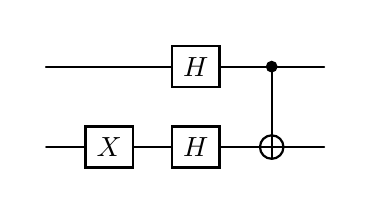
\begin{tikzpicture}
    \node[scale=1.0] {
      \begin{quantikz}
        \qw & \qw       & \gate{H} & \ctrl{1} & \qw \\
        \qw & \gate{X}  & \gate{H} & \targ{}  & \qw
      \end{quantikz}
    };
  \end{tikzpicture}\\
  Tukaj 3 unarna vrata (X, H) in ena binarna (C-NOT)
\end{frame}
\begin{frame}
  \frametitle{Težave}
  \pause
  \begin{itemize}
  \item Za večja vezja zelo nepregledna \pause
  \item Če dve vezji predstavljata isto transformacijo, ne poznamo (vedno) pravil, ki bi prvo pretvorila v drugo\pause
  \item Veliko trditev o kvantni mehaniki težko dokazati
  \end{itemize}
\end{frame}






\begin{frame}
  \frametitle{ZX-Račun}
  Vezje predstavimo kot graf. Definiramo dva tipa vozlišč: X pajek (rdeč) in Z pajek (zelen)\\
  Lahko imata poljubno število vhodov ali izhodov\\
  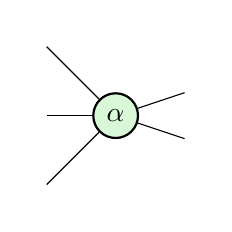
\begin{tikzpicture}
    %\begin{pgfonlayer}{nodelayer}
    \node (01) at (0, 0) {};
    \node (02) at (0, 1) {};
    \node (03) at (0, 2) {};
    \node [style=gn] (1) at (1.00, 1.00) {\(\alpha\)};
    \node (21) at (2, 0.66666) {};
    \node (22) at (2, 1.33333) {};
    %\end{pgfonlayer}
    %\begin{pgfonlayer}{edgelayer}
    \draw (01) to (1);
    \draw (02) to (1);
    \draw (03) to (1);
    \draw (1) to (21);
    \draw (1) to (22);
    %\end{pgfonlayer}
  \end{tikzpicture}\\
  Ta pajek ustreza preslikavi
  \begin{align*}
    \ket{00}\bra{000} + e^{i\alpha}\ket{11}\bra{111}
  \end{align*}
  Neformalno \(\bra{000}\) predstavlja kolikšen del vhodnega kubajta je \(\ket{000}\)
\end{frame}
\begin{frame}
  \frametitle{Več o pajkih}
  Rdeč pajek (X) se obnaša podobno kot Z pajek, le da v bazi \(\{\ket{-},\ket{+}\}\) namesto \(\{\ket0,\ket1\}\)\\
  Kadar je \(\alpha = 0\), oznake ne pišemo
  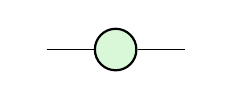
\begin{tikzpicture}
    \node (0) at (0,0) {};
    \node [style=gn] (1) at (1,0) {};
    \node (2) at (2,0) {};
    \draw (0) to (1);
    \draw (1) to (2);
  \end{tikzpicture}\\
  Očitno ne predstavljajo več unitarnih preslikav
\end{frame}
\begin{frame}
  \frametitle{Hadamardova vrata}
  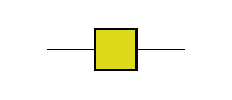
\begin{tikzpicture}
    \node (0) at (0,0) {};
    \node [style=had] (1) at (1,0) {};
    \node (2) at (2,0) {};
    \draw (0) to (1);
    \draw (1) to (2);
  \end{tikzpicture}\\
  Hadamardova vrata spreminjajo bazo. Lahko definiramo kot kompozicijo Z in X pajkov\\
  \vspace{3mm}
  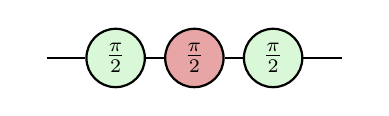
\begin{tikzpicture}
    \node (0) at (0.00, 0.00) {};
    \node [style=gn] (1) at (1, 0) {\(\frac\pi2\)};
    \node [style=rn] (2) at (2, 0) {\(\frac\pi2\)};
    \node [style=gn] (3) at (3, 0) {\(\frac\pi2\)};
    \node (4) at (4.00, 0.00) {};
    \draw (0) to (1);
    \draw (1) to (2);
    \draw (2) to (3);
    \draw (3) to (4);
  \end{tikzpicture}\\\pause{}
  Če imamo\vspace{3mm}\\
  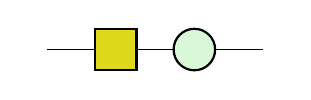
\begin{tikzpicture}
    \node (0) at (0,0) {};
    \node [style=had] (1) at (1,0) {};
    \node [style=gn] (2) at (2,0) {};
    \node (3) at (3,0) {};
    \draw (0) to (1);
    \draw (1) to (2);
    \draw (2) to (3);
  \end{tikzpicture}\\
  Lahko to pretvorimo v\vspace{3mm}\\
  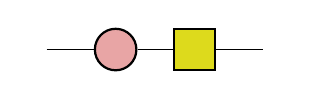
\begin{tikzpicture}
  \node (0) at (0,0) {};
  \node [style=rn] (1) at (1,0) {};
  \node [style=had] (2) at (2,0) {};
  \node (3) at (3,0) {};
  \draw (0) to (1);
  \draw (1) to (2);
  \draw (2) to (3);    
  \end{tikzpicture}
\end{frame}
\begin{frame}
  \frametitle{Povezava s kvantnimi vezji}
  V klasičnih vezjih vrata Z opazujejo spin v Z smeri.\\
  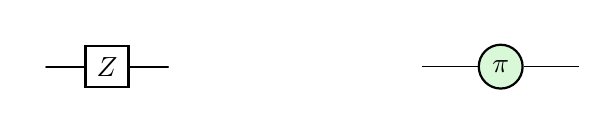
\begin{tikzpicture}
    \node[scale=1.0] (0,0) {
      \begin{quantikz}
        \qw & \gate{Z} & \qw
      \end{quantikz}
    };
    \node [style=gn] (1) at (5,0) {\(\pi\)};
    \draw (4,0) to (1);
    \draw (1) to (6,0);
  \end{tikzpicture}\\
  V ZX-računu to dosežemo s pajkom Z (in \(\alpha=\pi\)). Podobno za X smer.\\
  Vrata C-NOT postanejo\vspace{3mm}\\
  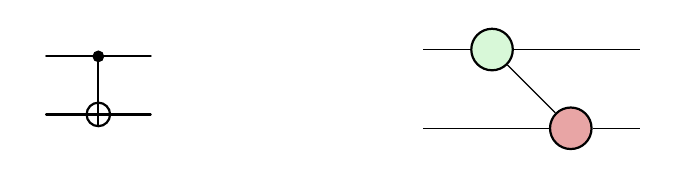
\begin{tikzpicture}
    \node (quantum) at (0,0.5) {
      \begin{quantikz}
        \qw & \ctrl{1} & \qw \\
        \qw & \targ{}  & \qw
      \end{quantikz}
    };
    \node (0) at (4, 0.00) {};
    \node (1) at (4, 1.00) {};
    \node [style=gn] (3) at (5, 1.00) {};
    \node [style=rn] (2) at (6, 0.00) {};
    \node (4) at (7, 0.00) {};
    \node (5) at (7, 1.00) {};
    \draw (0) to (2);
    \draw (1) to (3);
    \draw (2) to (3);
    \draw (2) to (4);
    \draw (3) to (5);
  \end{tikzpicture}\\
  Zgornji kubit pusti nespremenjen, spodnjega negira.
\end{frame}
\begin{frame}
  \frametitle{Pravila}
  Postavimo si nekaj aksiomov, ki grafično poenostavljajo vezja.

  Izbira ni unikatna! Z izbiro aksiomov izberemo delec ZX-računa. S tem izberemo kakšne kvantne sisteme simulira.

  Primer aksiomov nekega preprostega delca.
\end{frame}
\begin{frame}
  \frametitle{Aksiom: Pajki}
  Povezane pajke iste barve lahko združimo in seštejemo fazo.\\
  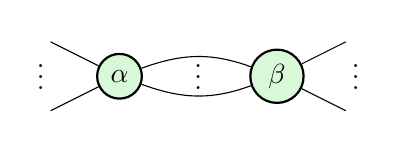
\begin{tikzpicture}
    \node (00) at (0,0) {};
    \node (dots1) at (0, 0.6) {\vdots};
    \node (01) at (0,1) {};
    \node [style=gn] (first) at (1,0.5) {\(\alpha\)};
    \node [style=gn] (second) at (3,0.5) {\(\beta\)};
    \node (dots3) at (2,0.6) {\vdots};
    \node (10) at (4,0) {};
    \node (dots2) at (4,0.6) {\vdots};
    \node (11) at (4,1) {};
    \draw (00) to (first);
    \draw (01) to (first);
    \draw (first) to [in=160, out=20] (second);
    \draw (first) to [in=200, out=340] (second);
    \draw (second) to (10);
    \draw (second) to (11);
  \end{tikzpicture}\\
  Je ekvivalenten\vspace{5mm}\\
  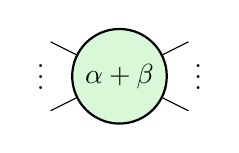
\begin{tikzpicture}
    \node (00) at (0,0) {};
    \node (dots1) at (0, 0.6) {\vdots};
    \node (01) at (0,1) {};
    \node [style=gn] (first) at (1,0.5) {\(\alpha+\beta\)};
    \node (10) at (2,0) {};
    \node (dots2) at (2,0.6) {\vdots};
    \node (11) at (2,1) {};
    \draw (00) to (first);
    \draw (01) to (first);
    \draw (first) to (10);
    \draw (first) to (11);
  \end{tikzpicture}
\end{frame}
\begin{frame}
  \frametitle{Aksiom: Identiteta}
  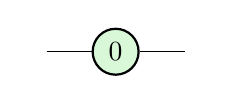
\begin{tikzpicture}
    \node (0) at (0,0) {};
    \node [style=gn] (g) at (1,0) {\(0\)};
    \node (1) at (2,0) {};
    \draw (0) to (g);
    \draw (g) to (1);
  \end{tikzpicture}\\
  Je ekvivalenten\vspace{5mm}\\
  \begin{tikzpicture}
    \node (0) at (0,0) {};
    \node (1) at (2,0) {};
    \draw (0) to (1);
  \end{tikzpicture}
\end{frame}
\begin{frame}
  \frametitle{Primer}
  Inverzne faze: \(-\alpha\) je inverzna faza od \(\alpha\)\vspace{5mm}\\
  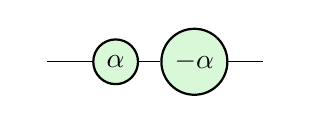
\begin{tikzpicture}
    \node (0) at (0,0) {};
    \node [style=gn] (1) at (1,0) {\(\alpha\)};
    \node [style=gn] (2) at (2,0) {\(-\alpha\)};
    \node (3) at (3,0) {};
    \draw (0) to (1);
    \draw (1) to (2);
    \draw (2) to (3);
  \end{tikzpicture}
\end{frame}
\begin{frame}
  \frametitle{Primer}
  Inverzne faze: \(-\alpha\) je inverzna faza od \(\alpha\)\vspace{5mm}\\
  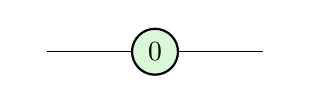
\begin{tikzpicture}
    \node (0) at (0,0) {};
    \node [style=gn] (1) at (1.5,0) {\(0\)};
    \node (3) at (3,0) {};
    \draw (0) to (1);
    \draw (1) to (3);
  \end{tikzpicture}
\end{frame}
\begin{frame}
  \frametitle{Primer}
  Inverzne faze: \(-\alpha\) je inverzna faza od \(\alpha\)\vspace{5mm}\\
  \begin{tikzpicture}
    \node (0) at (0,0) {};
    \node (3) at (3,0) {};
    \draw (0) to (3);
  \end{tikzpicture}
\end{frame}
\begin{frame}
  \frametitle{Odstranjevanje zank}
  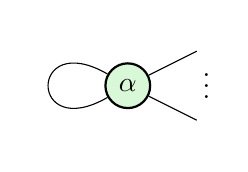
\begin{tikzpicture}
    \node [style=gn](main) at (1,0.5) {\(\alpha\)};
    \node (1) at (2,0) {};
    \node (dots) at (2,0.6) {\vdots};
    \node (2) at (2,1) {};
    \draw (main) to (1);
    \draw (main) to (2);
    \draw (main) to [in=150, out=210, looseness=10] (main);
  \end{tikzpicture}\\
  Je ekvivalentna\vspace{5mm}\\
  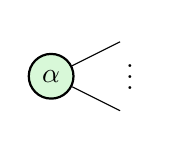
\begin{tikzpicture}
    \node [style=gn](main) at (1,0.5) {\(\alpha\)};
    \node (1) at (2,0) {};
    \node (dots) at (2,0.6) {\vdots};
    \node (2) at (2,1) {};
    \draw (main) to (1);
    \draw (main) to (2);
  \end{tikzpicture}
\end{frame}
\begin{frame}
  \frametitle{Aksiom: Bialgebra}
  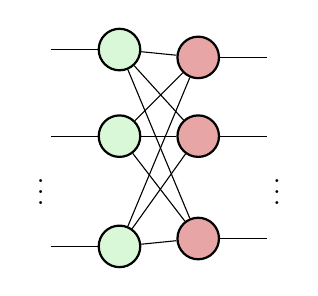
\begin{tikzpicture}
    \node (1s) at (0,0) {};
    \node (dotss) at (0, 0.8) {\vdots};
    \node (2s) at (0,1.4) {};
    \node (3s) at (0,2.5) {};
    \node [style=gn] (1g) at (1,0) {};
    \node [style=gn] (2g) at (1,1.4) {};
    \node [style=gn] (3g) at (1,2.5) {};
    \node [style=rn] (1r) at (2,0.1) {};
    \node [style=rn] (2r) at (2,1.4) {};
    \node [style=rn] (3r) at (2,2.4) {};
    \node (1e) at (3,0.1) {};
    \node (2e) at (3,1.4) {};
    \node (dotse) at (3, 0.8) {\vdots};
    \node (3e) at (3,2.4) {};
    \draw (1s) to (1g);
    \draw (2s) to (2g);
    \draw (3s) to (3g);
    \draw (1g) to (1r);
    \draw (1g) to (2r);
    \draw (1g) to (3r);
    \draw (2g) to (1r);
    \draw (2g) to (2r);
    \draw (2g) to (3r);
    \draw (3g) to (1r);
    \draw (3g) to (2r);
    \draw (3g) to (3r);
    \draw (1r) to (1e);
    \draw (2r) to (2e);
    \draw (3r) to (3e);
  \end{tikzpicture}\\
  Je ekvivalenten\vspace{5mm}\\
  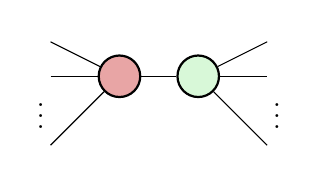
\begin{tikzpicture}
    \node (1s) at (0,0) {};
    \node (dotss) at (0, 0.6) {\vdots};
    \node (2s) at (0,1) {};
    \node (3s) at (0,1.5) {};
    \node [style=rn] (g) at (1, 1) {};
    \node [style=gn] (r) at (2, 1) {};
    \node (1e) at (3,0) {};
    \node (2e) at (3,1) {};
    \node (dotse) at (3, 0.6) {\vdots};
    \node (3e) at (3,1.5) {};
    \draw (1s) to (g);
    \draw (2s) to (g);
    \draw (3s) to (g);
    \draw (g) to (r);
    \draw (r) to (1e);
    \draw (r) to (2e);
    \draw (r) to (3e);
  \end{tikzpicture}
\end{frame}
\begin{frame}
  \frametitle{Primer: Kopiranje}
  Kopiranje (posebni primer bialgebre, ko ima pajek 0 povezav)\\
  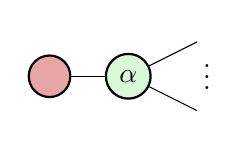
\begin{tikzpicture}
    \node [style=rn] (origin) at (0,0.5) {};
    \node [style=gn] (mid) at (1,0.5) {\(\alpha\)};
    \node (end) at (2,0) {};
    \node (dots) at (2,0.6) {\vdots};
    \node (end2) at (2,1) {};
    \draw (origin) to (mid);
    \draw (mid) to (end);
    \draw (mid) to (end2);
  \end{tikzpicture}\\
  postane\vspace{5mm}\\
  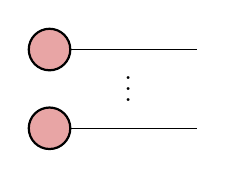
\begin{tikzpicture}
    \node [style=rn] (1) at (0,0) {};
    \node (1e) at (2,0) {};
    \node (dots) at (1,0.6) {\vdots};
    \node [style=rn] (2) at (0,1) {};
    \node (2e) at (2,1) {};
    \draw (1) to (1e);
    \draw (2) to (2e);
  \end{tikzpicture}\\
  To pravilo predstavlja nekvantne podatke.
\end{frame}
\begin{frame}
  \frametitle{Primer: Komplementarnost}
  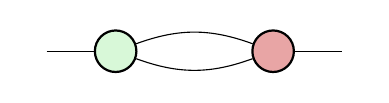
\begin{tikzpicture}
    \node (00) at (0,0.5) {};
    \node [style=gn] (first) at (1,0.5) {};
    \node [style=rn] (second) at (3,0.5) {};
    \node (10) at (4,0.5) {};
    \draw (00) to (first);
    \draw (first) to [in=160, out=20] (second);
    \draw (first) to [in=200, out=340] (second);
    \draw (second) to (10);
  \end{tikzpicture}
\end{frame}
\begin{frame}
  \frametitle{Primer: Komplementarnost}
  Samotni pajek je identiteta\\
  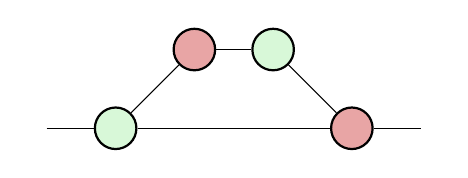
\begin{tikzpicture}
    \node (00) at (0,0) {};
    \node [style=rn] (imd) at (2,1) {};
    \node [style=gn] (imd2) at (3,1) {};
    \node [style=gn] (first) at (1,0) {};
    \node [style=rn] (second) at (4,0) {};
    \node (10) at (5,0) {};
    \draw (00) to (first);
    \draw (first) to (second);
    \draw (second) to (10);
    \draw (first) to (imd);
    \draw (imd) to (imd2);
    \draw (imd2) to (second);
  \end{tikzpicture}
\end{frame}
\begin{frame}
  \frametitle{Primer: Komplementarnost}
  Topološko ekvivalentno vezje je ekvivalentno\\
  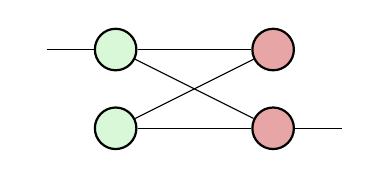
\begin{tikzpicture}
    \node (00) at (0,1) {};
    \node [style=rn] (imd) at (3,1) {};
    \node [style=gn] (imd2) at (1,0) {};
    \node [style=gn] (first) at (1,1) {};
    \node [style=rn] (second) at (3,0) {};
    \node (10) at (4,0) {};
    \draw (00) to (first);
    \draw (first) to (second);
    \draw (second) to (10);
    \draw (first) to (imd);
    \draw (imd) to (imd2);
    \draw (imd2) to (second);
  \end{tikzpicture}
\end{frame}
\begin{frame}
  \frametitle{Primer: Komplementarnost}
  Dodamo nove pajke, ki ne spremenijo vezja\\
  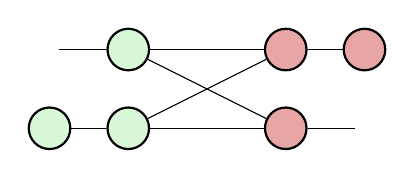
\begin{tikzpicture}
    \node (00) at (0,1) {};
    \node [style=gn] (newg) at (0,0) {};
    \node [style=rn] (newr) at (4,1) {};
    \node [style=rn] (imd) at (3,1) {};
    \node [style=gn] (imd2) at (1,0) {};
    \node [style=gn] (first) at (1,1) {};
    \node [style=rn] (second) at (3,0) {};
    \node (10) at (4,0) {};
    \draw (00) to (first);
    \draw (newr) to (imd);
    \draw (newg) to (imd2);
    \draw (first) to (second);
    \draw (second) to (10);
    \draw (first) to (imd);
    \draw (imd) to (imd2);
    \draw (imd2) to (second);
  \end{tikzpicture}
\end{frame}
\begin{frame}
  \frametitle{Primer: Komplementarnost}
  Uporabimo pravilo bialgebre\\
  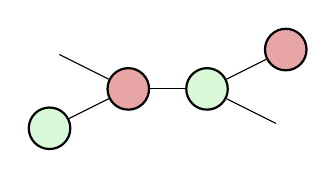
\begin{tikzpicture}
    \node (in) at (0,1) {};
    \node [style=gn] (ing) at (0,0) {};
    \node [style=rn] (mainr) at (1,0.5) {};
    \node [style=gn] (maing) at (2,0.5) {};
    \node (out) at (3,0) {};
    \node [style=rn] (outr) at (3,1) {};
    \draw (in) to (mainr);
    \draw (ing) to (mainr);
    \draw (mainr) to (maing);
    \draw (maing) to (out);
    \draw (maing) to (outr);
  \end{tikzpicture}
\end{frame}
\begin{frame}
  \frametitle{Primer: Komplementarnost}
  Spet topološko preuredimo za boljšo preglednost\\
  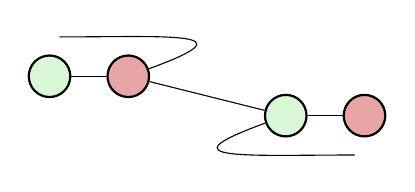
\begin{tikzpicture}
    \node (in) at (0,1.5) {};
    \node (out) at (4,0) {};
    \node [style=gn] (ing) at (0,1) {};
    \node [style=rn] (mainr) at (1,1) {};
    \node [style=gn] (maing) at (3,0.5) {};
    \node [style=rn] (outr) at (4,0.5) {};
    \draw (ing) to (mainr);
    \draw (mainr) to (maing);
    \draw (maing) to (outr);
    \draw (in) to [in=20, out=0, looseness=3] (mainr); %\draw (main) to [in=150, out=210, looseness=10] (main);
    \draw (maing) to [in=180, out=200, looseness=3] (out);
  \end{tikzpicture}
\end{frame}
\begin{frame}
  \frametitle{Primer: Komplementarnost}
  Uporabimo izrek za kloniranje na obeh straneh\\
  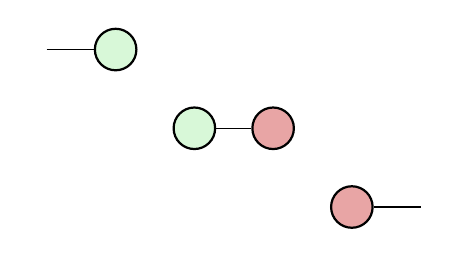
\begin{tikzpicture}
    \node (in) at (0,1) {};
    \node [style=gn] (ing) at (1,1) {};
    \node [style=gn] (middleg) at (2,0) {};
    \node [style=rn] (middler) at (3,0) {};
    \node [style=rn] (outr) at (4,-1) {};
    \node (out) at (5,-1) {};
    \draw (in) to (ing);
    \draw (middleg) to (middler);
    \draw (outr) to (out);
  \end{tikzpicture}
\end{frame}
\begin{frame}
  \frametitle{Primer: Komplementarnost}
  Odstranimo nepovezan del in dobimo, da se\\
  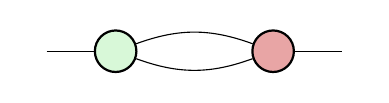
\begin{tikzpicture}
    \node (00) at (0,0.5) {};
    \node [style=gn] (first) at (1,0.5) {};
    \node [style=rn] (second) at (3,0.5) {};
    \node (10) at (4,0.5) {};
    \draw (00) to (first);
    \draw (first) to [in=160, out=20] (second);
    \draw (first) to [in=200, out=340] (second);
    \draw (second) to (10);
  \end{tikzpicture}\\
  poenostavi v \vspace{5mm}\\
  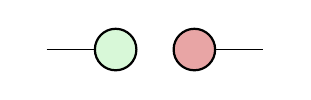
\begin{tikzpicture}
    \node (0) at (0,0) {};
    \node [style=gn] (gn) at (1,0) {};
    \node [style=rn] (rn) at (2,0) {};
    \node (1) at (3,0) {};
    \draw (0) to (gn);
    \draw (rn) to (1);
  \end{tikzpicture}

\end{frame}
\begin{frame}
  \frametitle{Aksiom: Zamenjava barve}
  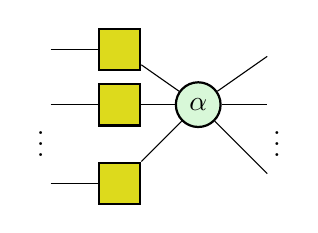
\begin{tikzpicture}
    \node (1s) at (0,0) {};
    \node (dotss) at (0, 0.6) {\vdots};
    \node (2s) at (0,1) {};
    \node (3s) at (0,1.7) {};
    \node [style=had] (1h) at (1,0) {};
    \node [style=had] (2h) at (1,1) {};
    \node [style=had] (3h) at (1,1.7) {};
    \node [style=gn] (main) at (2,1) {\(\alpha\)};
    \node (1e) at (3,0) {};
    \node (2e) at (3,1) {};
    \node (dotse) at (3, 0.6) {\vdots};
    \node (3e) at (3,1.7) {};
    \draw (1s) to (1h);
    \draw (2s) to (2h);
    \draw (3s) to (3h);
    \draw (1h) to (main);
    \draw (2h) to (main);
    \draw (3h) to (main);
    \draw (main) to (1e);
    \draw (main) to (2e);
    \draw (main) to (3e);
  \end{tikzpicture}\\
  Je ekvivalentno\vspace{5mm}\\
  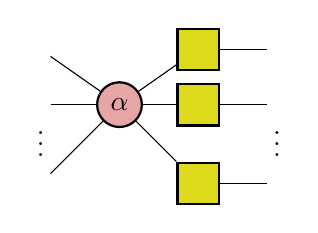
\begin{tikzpicture}
    \node (1s) at (0,0) {};
    \node (dotss) at (0, 0.6) {\vdots};
    \node (2s) at (0,1) {};
    \node (3s) at (0,1.7) {};
    \node [style=had] (1h) at (2,0) {};
    \node [style=had] (2h) at (2,1) {};
    \node [style=had] (3h) at (2,1.7) {};
    \node [style=rn] (main) at (1,1) {\(\alpha\)};
    \node (1e) at (3,0) {};
    \node (2e) at (3,1) {};
    \node (dotse) at (3, 0.6) {\vdots};
    \node (3e) at (3,1.7) {};
    \draw (1s) to (main);
    \draw (2s) to (main);
    \draw (3s) to (main);
    \draw (1h) to (main);
    \draw (2h) to (main);
    \draw (3h) to (main);
    \draw (1h) to (1e);
    \draw (2h) to (2e);
    \draw (3h) to (3e);
  \end{tikzpicture}
\end{frame}
\begin{frame}
  \frametitle{kvantni orakelj}
  Skoraj vsak zanimiv problem v računalništvu lahko prevedemo v SAT problem.

  Iščemo vrednost \(x\) funkcijske preslikave
  \begin{align*}
    f:\{0,1\}^n\to \{0,1\}
  \end{align*}
  za katero
  \begin{align*}
    f(x) = 1
  \end{align*}
\end{frame}
\begin{frame}
  \frametitle{kvantni orakelj}
  Predstavili jo bomo z trapezom\\
  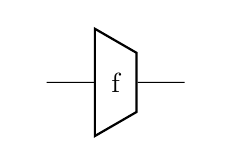
\begin{tikzpicture}
    \node (in) at (0,0) {};
    \node [style=func] (f) at (1,0) {f};
    \node (out) at (2,0) {};
    \draw (in) to (f);
    \draw (f) to (out);
  \end{tikzpicture}\\
  V splošnem ta funkcija ni unitarna!
\end{frame}
\begin{frame}
  \frametitle{Pogoj homomorfizma}
  Za funkcijske preslikave zahtevamo, da je\\
  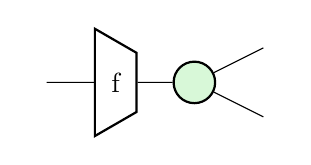
\begin{tikzpicture}
    \node (in) at (0,0) {};
    \node [style=func] (f) at (1,0) {f};
    \node [style=gn] (out) at (2,0) {};
    \node (up) at (3,0.5) {};
    \node (down) at (3,-0.5) {};
    \draw (in) to (f);
    \draw (f) to (out);
    \draw (out) to (up);
    \draw (out) to (down);
  \end{tikzpicture}\\
  enak\vspace{5mm}\\
  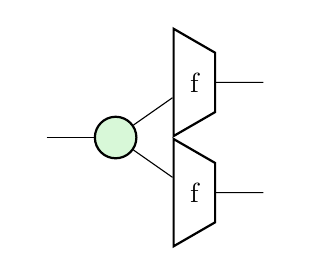
\begin{tikzpicture}
    \node (in) at (0,0) {};
    \node [style=func] (fu) at (2,0.7) {f};
    \node [style=func] (fd) at (2,-0.7) {f};
    \node [style=gn] (out) at (1,0) {};
    \node (up) at (3,0.7) {};
    \node (down) at (3,-0.7) {};
    \draw (in) to (out);
    \draw (fu) to (out);
    \draw (fd) to (out);
    \draw (fu) to (up);
    \draw (fd) to (down);
  \end{tikzpicture}

  To vedno lahko dosežemo tako, da jo zapišemo kot linearno preslikavo.
\end{frame}
\begin{frame}
  \frametitle{unitarni kvantni orakelj}
  Vsako tako funkcijo lahko pretvorimo v unitarno
  
  Definiramo si iteriran pajek\\
  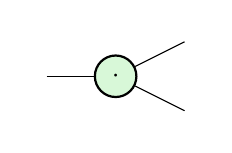
\begin{tikzpicture}
    \node (s) at (0,0) {};
    \node [style=gn] (a) at (1,0) {\(\cdot\)};
    \node (eu) at (2,0.5) {};
    \node (ed) at (2,-0.5) {};
    \draw (s) to (a);
    \draw (a) to (eu);
    \draw (a) to (ed);
  \end{tikzpicture}\\
  Enak pa naj bo \(n\) kopijam samega sebe brez pike. 
\end{frame}
\begin{frame}
  \frametitle{unitarni kvantni orakelj}
  Primer za \(n=2\)\\
  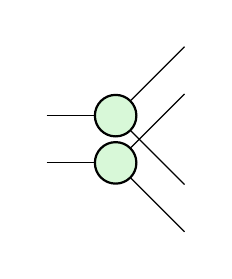
\begin{tikzpicture}
    \node (s) at (0,0) {};
    \node (s2) at (0,0.6) {};
    \node [style=gn] (a) at (1,0) {};
    \node (eu) at (2,1) {};
    \node (ed) at (2,-1) {};
    \node [style=gn] (a2) at (1,0.6) {};
    \node (eu2) at (2,1.6) {};
    \node (ed2) at (2,-0.4) {};
    \draw (s) to (a);
    \draw (a) to (eu);
    \draw (a) to (ed);
    \draw (s2) to (a2);
    \draw (a2) to (eu2);
    \draw (a2) to (ed2);
  \end{tikzpicture}\\

  Vrednost \(n\) je implicitno število vhodov funkcije
\end{frame}
\begin{frame}
  \frametitle{unitarni kvantni orakelj}
  Preslikava\vspace{5mm}\\
  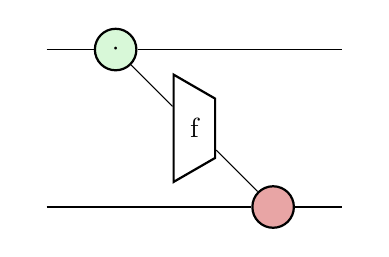
\begin{tikzpicture}
    \node (sr) at (0,0) {};
    \node (sg) at (0,2) {};
    \node [style=gn] (g) at (1,2) {\(\cdot\)};
    \node [style=func] (f) at (2,1) {f};
    \node [style=rn] (r) at (3,0) {};
    \node (eg) at (4,2) {};
    \node (er) at (4,0) {};
    \draw (sg) to (g);
    \draw (g) to (f);
    \draw (f) to (r);
    \draw (g) to (eg);
    \draw (sr) to (r);
    \draw (r) to (er);
  \end{tikzpicture}\\
  je unitarna.
\end{frame}

\end{document}